% ============================================================================
%  Project Specification and Preliminary Report
%  FYP 2026-27, Glasgow College UESTC (Hainan) — UESTCHN4008P
%  Build:  xelatex -> bibtex -> xelatex -> xelatex
% ============================================================================
\documentclass[10pt,a4paper]{article}

\usepackage[UTF8]{ctex}
\usepackage{fontspec}
\setmainfont{Times New Roman}
\setsansfont{Arial}
\setmonofont{Consolas}

\usepackage[a4paper,top=1.8cm,bottom=1.7cm,left=2.1cm,right=2.1cm]{geometry}
\usepackage{graphicx}
\usepackage{float}
\usepackage{booktabs}
\usepackage{array}
\usepackage{amsmath}
\usepackage{xcolor}
\usepackage{enumitem}
\usepackage{caption}
\usepackage{fancyhdr}
\usepackage[hidelinks]{hyperref}
\usepackage{parskip}
\setlength{\parskip}{3pt plus 1pt}
\setlength{\parindent}{0pt}
\usepackage{tikz}
\usetikzlibrary{arrows,positioning,fit,backgrounds}
\usepackage[htt]{hyphenat}
\setlength{\emergencystretch}{2.5em}

\captionsetup{font=small,labelfont=bf,skip=4pt}
\setlist[itemize]{leftmargin=1.3em,topsep=2pt,itemsep=1pt}
\setlist[enumerate]{leftmargin=1.6em,topsep=2pt,itemsep=1pt}

\pagestyle{fancy}
\fancyhf{}
\fancyhead[L]{\small\itshape Project Specification and Preliminary Report}
\fancyhead[R]{\small\itshape Xu Yuxuan, 2959485}
\fancyfoot[C]{\small\thepage}
\renewcommand{\headrulewidth}{0.4pt}

\newcommand{\code}[1]{\texttt{\small #1}}

\begin{document}

% ---------------------------------------------------------------------------
%  Cover block (template fields)
% ---------------------------------------------------------------------------
\begin{center}
  {\large\bfseries Design and Development of an AI-Enabled Smart Electric Vehicle\\
   Charging and Energy Management Platform}\\[4pt]
  {\normalsize Project Specification and Preliminary Report}\\[2pt]
  {\small Sub-project 1: EV Charging Data Analysis and Demand Forecasting}\\[6pt]
  {\small University of Glasgow \,|\, Glasgow College UESTC, Hainan \,|\, UESTCHN4008P}
\end{center}

\vspace{-2pt}
{\small
\renewcommand{\arraystretch}{1.15}
\begin{tabular}{@{}p{3.5cm}p{6.6cm}p{2.9cm}p{1.9cm}@{}}
\toprule
Student name & Xu Yuxuan & Matriculation & 2959485 \\
UESTC student number & 2959485 & Academic year & 2026--27 \\
First supervisor & Dr Amer Ghias & Placement company & --- \\
Degree programme & Electronics and Information Engineering & & \\
Working title & AI-enabled smart EV charging and energy management platform & & \\
\bottomrule
\end{tabular}
}

\vspace{4pt}
{\footnotesize\itshape
I affirm that this submission is all my own work in accordance with the University of Glasgow and
UESTC Regulations, and the James Watt School of Engineering requirements. \hfill Signed:
\underline{\hspace{4.2cm}} \quad Date: \underline{\hspace{2.2cm}}}

% ---------------------------------------------------------------------------
\section{Project Description and Background}

\begin{center}
\resizebox{\textwidth}{!}{%
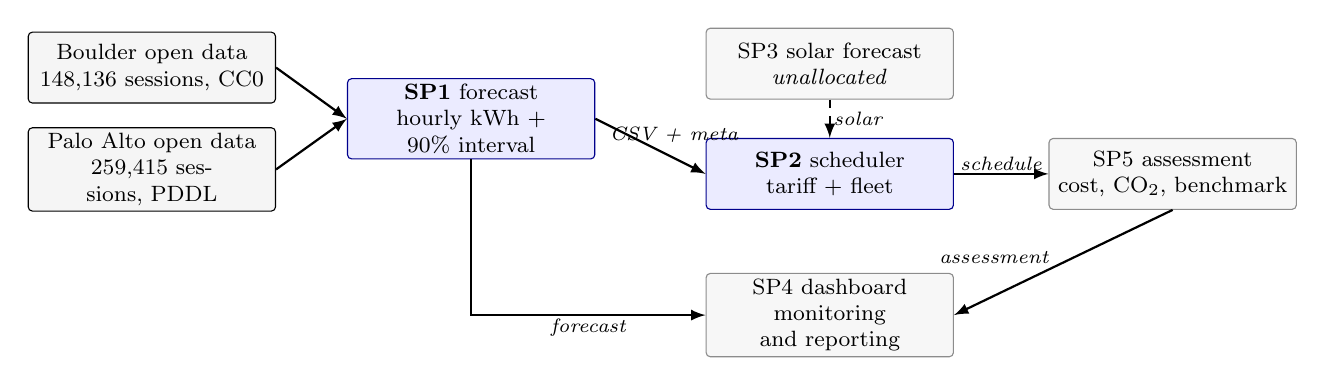
\begin{tikzpicture}[
  font=\footnotesize,
  box/.style={draw, rounded corners=1.5pt, align=center, minimum height=9mm,
              text width=30mm, inner sep=2pt, fill=white},
  data/.style={box, fill=black!4},
  own/.style={box, fill=blue!8, draw=blue!55!black},
  other/.style={box, fill=black!3, draw=black!45},
  ar/.style={-latex, thick},
  lab/.style={font=\scriptsize\itshape, inner sep=1pt}
]
\node[data] (b) {Boulder open data\\148{,}136 sessions, CC0};
\node[data, below=3mm of b] (p) {Palo Alto open data\\259{,}415 sessions, PDDL};
\node[own, right=9mm of b, yshift=-6.5mm] (sp1) {\textbf{SP1} forecast\\hourly kWh + 90\% interval};
\node[other, right=14mm of sp1, yshift=7mm] (sp3) {SP3 solar forecast\\\emph{unallocated}};
\node[own, right=14mm of sp1, yshift=-7mm] (sp2) {\textbf{SP2} scheduler\\tariff + fleet};
\node[other, right=12mm of sp2] (sp5) {SP5 assessment\\cost, CO$_2$, benchmark};
\node[other, below=8mm of sp2] (sp4) {SP4 dashboard\\monitoring and reporting};

\draw[ar] (b.east) -- (sp1.west);
\draw[ar] (p.east) -- (sp1.west);
\draw[ar] (sp1.east) -- node[lab, above, xshift=3mm]{CSV + meta} (sp2.west);
\draw[ar, dashed] (sp3.south) -- node[lab, right]{solar} (sp2.north);
\draw[ar] (sp2.east) -- node[lab, above]{schedule} (sp5.west);
\draw[ar] (sp5.south) -- node[lab, above left, pos=0.55]{assessment} (sp4.east);
\draw[ar] (sp1.south) |- node[lab, pos=0.75, below]{forecast} (sp4.west);
\end{tikzpicture}}
\captionof{figure}{Platform architecture. Blue boxes are the components this report builds; grey
boxes are the other sub-projects, shown only to fix the interfaces.}
\label{fig:arch}
\end{center}

Electric vehicle (EV) adoption is adding load to distribution networks faster than network capacity
is being reinforced, and the timing of that load is set by drivers rather than by the network.
Uncoordinated charging concentrates demand in the hours when vehicles are parked and their owners
are available to plug in, which raises peak demand, raises the price paid for energy, and can force
curtailment of renewable generation that would otherwise have been absorbed. Coordinated charging
inverts the problem: the same energy can be delivered at a different time, so peak demand falls
without any reduction in the service provided. The platform in this project implements that
inversion as a software pipeline: forecast the demand, schedule it against a tariff and a
generation profile, display the result, and quantify what it saved.

The platform is split into five sub-projects with fixed interfaces. Sub-project 1 (SP1, this
report) converts charging session records into an hourly demand series and forecasts the next 24
hours with a prediction interval. SP2 schedules that demand against a time-of-use tariff and a
fleet of vehicles. SP3 supplies a solar generation forecast which SP2 may consume; it is not yet
allocated to a student, and the interface is defined so that its absence is treated as zero solar
rather than as a blocker. SP4 is the monitoring dashboard that consumes every other sub-project's
output file. SP5 assesses the economic and environmental outcome. Figure~\ref{fig:arch} shows the
data flow and the contract file carried on each edge.

The forecasting layer is the one that determines whether the rest of the platform can be evaluated
at all: a schedule is only as good as the demand it is built on, and a dispatch constraint has to
hold against the upper end of the forecast interval rather than against a point forecast. The
importance is measurable rather than rhetorical. On the primary site used in this report, if every
session charges as soon as it connects, the hourly peak reaches 362.5\,kWh against a forecast peak
of 94.5\,kWh, an amplification of 3.84, while total energy delivered moves by 0.05\,\%. The saving
available to the platform therefore lies in moving load in time, not in reducing it, and the size
of that saving is set by how well demand can be predicted and how tightly its uncertainty can be
bounded.


% ---------------------------------------------------------------------------
\section{Literature Review}

\subsection{Forecasting EV charging demand}

Published work on station-level load forecasting divides into model-family comparisons and one
systematised review, and the model family that wins depends on the data rather than on the
architecture. Zhu et al.~\cite{Zhu2019ShortTermEVLoadDL} compare four deep architectures on hourly
station load and report a gated recurrent unit network as the best performer, framing the problem
as a large fleet power draw driven by stochastic driver behaviour.
Vishnu et al.~\cite{Vishnu2023ShortTermEVLoadTSMLDL} compare an auto-regressive model, support
vector regression and an LSTM on Adaptive Charging Network data, report the LSTM as best with
MAE 4\,kW and RMSE 5.9\,kW, and provide the most concrete published error figure in this strand.
Zhang et al.~\cite{Zhang2022MCCNNTCN} combine a multi-channel convolutional network with a temporal
convolutional network and add meteorological and calendar covariates, improving on an ANN by
14.09\,\%, on an LSTM by 25.13\,\% and on a TCN by 4.48\,\%. Ge et
al.~\cite{Ge2020SpatialTemporalEVLoadProfile} instead use a random forest with harmony-search
tuning and construct the spatial-temporal load of vehicle clusters bottom-up.
Alaraj et al.~\cite{Alaraj2025MLChargingDemandReview} survey the field and state the ordering that
this project adopts: unmanaged adoption risks network instability, smart charging mitigates it, and
smart charging presupposes an accurate forecast.

\begin{table}[H]
\centering
\caption{Representative forecasting studies and what they establish for this project.}
\label{tab:lit}
\small
\renewcommand{\arraystretch}{1.15}
\begin{tabular}{@{}p{3.3cm}p{3.6cm}p{3.0cm}p{5.0cm}@{}}
\toprule
Study & Data and level & Model & What it settles here \\
\midrule
Zhu et al.~\cite{Zhu2019ShortTermEVLoadDL} & Station, hourly & GRU & Recurrent models are competitive at station level \\
Vishnu et al.~\cite{Vishnu2023ShortTermEVLoadTSMLDL} & ACN, station & LSTM & MAE 4\,kW; a reference error figure from the same data family \\
Zhang et al.~\cite{Zhang2022MCCNNTCN} & Urban station, 15\,min & CNN + TCN & Calendar and weather covariates improve accuracy \\
Ge et al.~\cite{Ge2020SpatialTemporalEVLoadProfile} & Cluster & Random forest & Spatial aggregation needs a bottom-up construction \\
Alaraj et al.~\cite{Alaraj2025MLChargingDemandReview} & Review & --- & Forecast first, schedule second \\
\bottomrule
\end{tabular}
\end{table}

\subsection{From session records to hourly load profiles}

The project's central data-engineering assumption is that a table of sessions, each carrying a
connection time, a disconnection time and a metered energy quantity, can be turned into an hourly
power profile. Yi and Scoffield~\cite{Yi2018ResidentialLoadProfileGeneration} estimate the
distribution of charging duration conditional on parking duration and generate synthetic behaviour
that preserves the parking-to-travel dependency. Uimonen and
Lehtonen~\cite{Uimonen2020OfficeBuildingOccupancy} derive office-building profiles from measured
charger occupancy, the closest published analogue to the workplace site used here.
Munkhammar et al.~\cite{Munkhammar2014BernoulliPEVCharging} reduce a Monte Carlo state-of-charge
simulation to hour-by-hour Bernoulli distributions of plug-in status and show that the aggregate
over many vehicles is approximately normal, which is the formal basis for turning per-vehicle
plug-in indicators into a fleet profile. Lahariya et
al.~\cite{Lahariya2020SyntheticDataGenerator} model arrivals as a Poisson-like process with
connection time dependent on arrival time, and von
Hoffen~\cite{vonHoffen2016ChargingTransactionAnalytics} makes the complementary point that
transaction records acquire analytical value only after enrichment with context. The consequence
for this project is that charging duration is modelled as a function of occupancy rather than as a
constant rate, which is why a session's metered energy is spread across its charging window in
proportion to overlap instead of being divided by a rated power.

\subsection{Tariffs, scheduling and peak reduction}

Chen et al.~\cite{Chen2012ValleyFilling} formulate joint optimal power flow and EV charging for a
fleet with heterogeneous charging-rate limits and characterise the optimal offline schedule as a
valley-filling profile, giving both a centralised and a decentralised online algorithm that tracks
it; this is the benchmark against which a scheduling heuristic can be judged approximately optimal.
Ramadan et al.~\cite{Ramadan2018PeakShavingValleyFilling} solve the related peak-shaving problem
with particle swarm optimisation and allow vehicle-to-grid discharge during peaks. On the tariff
side, Davis and Bradley~\cite{Davis2012TOURatesEfficacy} test whether time-of-use rates actually
shift charging and find that for plug-in hybrids the extra fuelling cost of charging off-peak can
cancel the incentive, so tariff response is not free and a cost-saving result that assumes it is
free overstates the benefit. Szinai et al.~\cite{Szinai2020ReducedGridOperatingCosts} link mobility
and dispatch models for California and report that 0.95--5 million managed vehicles avoid
USD 120--690 million in annual operating costs, up to 10\,\%, and cut renewable curtailment by up
to 40\,\%, while noting that overnight time-of-use charging increases curtailment at similar cost
savings. Dixon et al.~\cite{Dixon2020MinimiseEmissionsWindCurtailment} schedule against grid carbon
intensity and wind availability, reducing average charging emissions from 35--56 to
28--40\,gCO\textsubscript{2}/km. Cost and curtailment are therefore separately measurable
objectives that can move in opposite directions, and a schedule has to state which one it
optimises.

\subsection{Open data and measured grid impact}

Amara-Ouali et al.~\cite{AmaraOuali2021EVLoadOpenDataReview} survey open data for reproducible EV
load research, searching more than 860 repositories and returning roughly 60 datasets, and motivate
the survey by the field's shortage of charging-station data of realistic consistency. That finding
framed the dataset choice made here: official municipal releases were selected on provenance, a
public-domain or open licence, metered energy per session, and downloadable access without
registration. Li et al.~\cite{Li2025UrbanEV} publish UrbanEV, covering charging-space availability
and electricity consumption in Shenzhen at hourly resolution for more than 20{,}000 stations, and
Lee et al.~\cite{Lee2021ACNSim} present ACN-Sim, which also serves as the DOI-bearing citation for
the Adaptive Charging Network dataset. On the impact side, Powell et
al.~\cite{Powell2022ChargingInfrastructureGridImpacts} evaluate charging demand against a 2035
economic dispatch for the Western Interconnection and find peak net demand rising by up to
25\,\% under forecast adoption and 50\,\% in a full-electrification stress test, with the
counter-intuitive result that locally optimised charging combined with a high share of home
charging can strain the grid, while uncontrolled \emph{daytime} charging reduces storage, ramping
and emissions. Verma et al.~\cite{Verma2021ReviewImpactsDistributionNetwork} review
distribution-network impacts across penetration levels, supporting the treatment of impact as a
function of fleet size rather than as a fixed property of EVs.

\subsection{Significance and the gap addressed}

Three conclusions follow from the review and shape the specification. First, one-hour resolution
with a rolling-origin out-of-sample protocol and explicit naive baselines is the minimum design
under which a reported accuracy means anything; the reviewed papers mostly compare model families
against each other, and a learned model that does not beat persistence has demonstrated nothing.
Second, published absolute errors come from other datasets and larger sites, so they are context
rather than targets. Third, session-level open data with metered energy is scarce, and the Chinese
official route was closed after verification: the national charging platform publishes monthly
aggregates for members, not per-session records, so the forecasting work rests on two municipal
releases.

What is missing in that literature, and what this project therefore specifies, is a forecasting
layer built on open municipal session data that (i) reports accuracy against naive baselines
rather than only against other learned models, (ii) carries a calibrated prediction interval that
is evaluated by its coverage rather than assumed, and (iii) demonstrates that the result transfers
to a second city without retuning. The next section turns the gap into objectives.

% ---------------------------------------------------------------------------
\section{SMART Objectives}

Four objectives are specified. Each states a measurable target and the date by which it is met, and
each maps to a task in the work plan of Section~\ref{sec:plan}.

\begin{enumerate}[label=O\arabic*.]
  \item \textbf{A reproducible demand series from open session data.} By 30 October 2026, convert
        the two official municipal session datasets into gap-free hourly demand series in UTC, with
        a contract-validated CSV plus metadata sidecar and at least 50 automated tests covering
        ingestion, aggregation and time-zone handling. \emph{Achieved: 77 tests pass; both series
        are produced by one command from a checksummed download.}
  \item \textbf{Day-ahead forecasts that beat persistence on both sites.} By 31 January 2027,
        produce 1--24\,h forecasts that reduce WAPE against the naive same-hour-yesterday baseline
        by at least 15\,\% on the primary site and by at least 10\,\% on the validation site, with
        measured coverage of the nominal 90\,\% interval within $\pm$3 percentage points.
        \emph{Partially achieved: 19\,\% and 18\,\% reductions, coverage 91.0\,\% and 90.5\,\%.}
  \item \textbf{A quantified peak-shifting target for the scheduler.} By 30 April 2027, quantify,
        for the primary site, the peak reduction and cost difference between uncontrolled charging
        and a schedule built on the forecast, and deliver both series to SP5 for the assessment.
        \emph{In progress: the uncontrolled baseline is built; the scheduled series depends on SP2.}
  \item \textbf{An interface that other sub-projects consume unchanged.} By 30 April 2027, deliver
        the forecast as a contract file that SP2, SP4 and SP5 read without transformation, with the
        interval columns populated and the method recorded in the sidecar.
        \emph{Partially achieved: the contract file and sidecar exist and are versioned.}
\end{enumerate}

The key contributions are the use of official municipal session data as a forecasting basis where
the field mostly relies on proprietary or single-site records, a direct multi-horizon formulation in
which the forecast step is an input feature rather than a recursion, and an interval that is
evaluated by its coverage instead of being asserted.

% ---------------------------------------------------------------------------
\section{Technical Background}

\subsection{Hypothesis and method}

The hypothesis is that aggregate charging demand at a municipal or workplace site is governed by
calendar structure and by the recent level of demand, so that a gradient-boosted model on
target-hour calendar values plus forecast-origin lags, with the forecast horizon supplied as a
feature, predicts one to twenty-four hours ahead more accurately than persistence at every horizon.
Two consequences follow. Because the horizon is a feature, one model serves all horizons and needs
no recursion, which removes the error compounding that a one-step model accumulates when iterated.
Because every feature is either a calendar value of the \emph{target} interval or a lag anchored at
the \emph{origin}, no information from the future can enter the model; a regression test recomputes
each lag from the raw series and fails if any feature can see its own target.

\subsection{Data and derivation}

Two official municipal releases are used. The City of Boulder, Colorado, publishes 148{,}136
charging transactions at 50 city-owned Level-2 stations between January 2018 and December 2023,
with metered energy per session, under CC0; it is the primary site and supplies 1.253\,GWh. The
City of Palo Alto, California, publishes 259{,}415 sessions at 47 stations between July 2011 and
January 2021 under the PDDL, supplying 2.216\,GWh; it is used only for validation. Both are
session-level records with connection time, disconnection time and metered energy, which is the
minimum schema the derivation needs.

Each session's metered energy is spread over the hourly intervals it actually overlaps, in
proportion to the overlap, and the timeline is closed into a gap-free hourly grid. This is the
occupancy-conditional treatment argued for by~\cite{Yi2018ResidentialLoadProfileGeneration} and
\cite{Uimonen2020OfficeBuildingOccupancy}, with one limitation inherited from the source: the
records carry no within-session power taper, so a constant rate is assumed inside a session. The
assumption is recorded in the output metadata rather than left implicit.

\subsection{Evaluation and interval construction}

Seven models are scored: three naive baselines (same hour yesterday, same hour last week, and an
hour-of-week profile) and four learned models (ridge regression, random forest, gradient boosting
and XGBoost). Evaluation is a rolling-origin backtest in which every model is retrained at every
origin using only targets strictly before that origin, and each origin forecasts the following
24 hours; origins are anchored to local midnight, so each is a genuine day-ahead forecast. Accuracy
is reported as WAPE, the total absolute error divided by total demand, which stays stable when many
intervals carry near-zero demand, alongside MAE, RMSE and $R^2$. The interval is empirical:
$\hat{y} \pm 1.645\,\sigma$, where $\sigma$ is the residual standard deviation at the same horizon
in the backtest, clipped at zero because demand cannot be negative.

\subsection{Preliminary results}

\begin{table}[H]
\centering
\caption{Rolling-origin results, targets strictly out of sample. Boulder: 25 origins, 600 hours.
Palo Alto: 14 origins, 336 hours. The interval is nominal 90\,\%.}
\label{tab:results}
\small
\renewcommand{\arraystretch}{1.15}
\begin{tabular}{@{}lrr@{}}
\toprule
Metric & Boulder (primary) & Palo Alto (validation) \\
\midrule
WAPE, gradient boosting & 0.292 & 0.549 \\
WAPE, naive same hour yesterday & 0.360 & 0.670 \\
Relative reduction in WAPE & 19\,\% & 18\,\% \\
MAE (kWh per hour) & 8.37 & 7.02 \\
RMSE (kWh per hour) & 11.39 & 9.70 \\
$R^2$ & 0.763 & 0.466 \\
Measured coverage of the 90\,\% interval & 91.0\,\% & 90.5\,\% \\
\bottomrule
\end{tabular}
\end{table}

On the primary site the gradient-boosted model reaches a WAPE of 0.292 against 0.360 for the naive
daily baseline, a reduction of 19\,\%, with $R^2$ of 0.763 and a measured interval coverage of
91.0\,\% against a nominal 90\,\%; the mean interval width is 33.2\,kWh per hour. The same
pipeline, with no parameter changed, reaches 0.549 against 0.670 on the validation site, still a
reduction of 18\,\%, at 90.5\,\% coverage. The normalised error is higher on the validation site
while the absolute error per hour is comparable (7.02 against 8.37\,kWh), because the two windows
differ in scale and in period; the absolute figures are therefore not comparable across sites, and
the claim made here is the within-site relative gain, which repeats at 18\,\%. That repetition is
the evidence that the gain comes from the method rather than from tuning.
Figure~\ref{fig:fc} shows the last week of the evaluation window.

\begin{figure}[tbp]
\centering
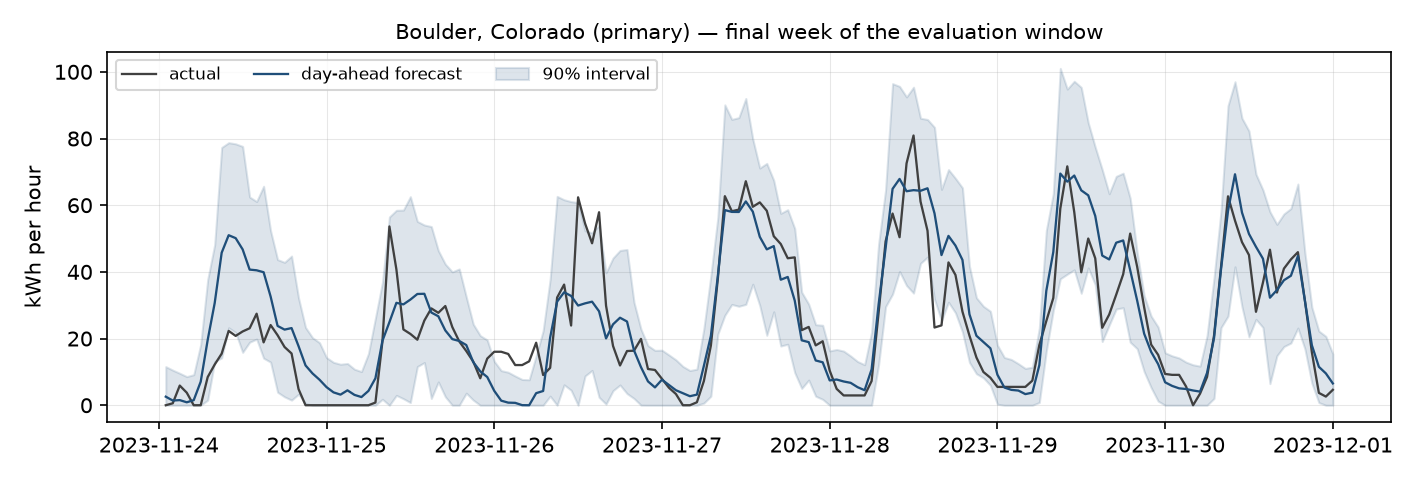
\includegraphics[width=0.94\textwidth]{../phase1-report/figures/sp1-forecast-vs-actual.png}
\caption{Metered demand, day-ahead forecast and the 90\,\% prediction interval over the final week
of the evaluation window on the primary site. The band widens where demand is volatile because it
is built from the residual quantiles of the backtest at each horizon.}
\label{fig:fc}
\end{figure}

Two properties of the data constrain the platform that consumes these forecasts. Both sites peak in
the middle of the working day, at 11:00 in Boulder and 12:00 in Palo Alto, and bottom out at 04:00
with a peak-to-trough ratio of about nineteen; there is no residential evening peak, because this
is public charging rather than home charging. A scheduler that assumes the evening peak of the
project brief would therefore optimise the wrong hours, which is a finding the Phase-3 design has
to carry.

% ---------------------------------------------------------------------------
\section{References}

\bibliographystyle{unsrt}
\bibliography{../literature-review/references}

% ---------------------------------------------------------------------------
\clearpage
\section{Measurable Outcomes and Work Plan}\label{sec:plan}

\begin{table}[H]
\centering
\caption{Main tasks, measurable targets and dates. Type: S = software, D = data, A = analysis,
T = theoretical.}
\label{tab:plan}
\small
\renewcommand{\arraystretch}{1.12}
\begin{tabular}{@{}p{0.6cm}p{6.6cm}p{6.0cm}p{2.1cm}@{}}
\toprule
Type & Task & Measurable target & Due \\
\midrule
D & Acquire and register official session datasets & Two series reproducible from a checksummed download & Sep 2026 \\
S & Session-to-hourly pipeline with contract IO & Gap-free hourly CSV plus metadata, $\geq$50 tests & Oct 2026 \\
S & Feature set, direct multi-horizon models, backtest & WAPE reported against three naive baselines & Oct 2026 \\
A & Interval construction and coverage check & Measured coverage within $\pm$3\,pp of nominal & Nov 2026 \\
A & Cross-site validation without retuning & Relative WAPE reduction $\geq$10\,\% on site 2 & Nov 2026 \\
S & Tariff-aware features and interface freeze & Contract v2 consumed by SP2 without change & Dec 2026 \\
A & Interim report and presentation & Submitted 8 Jan; presented 11--22 Jan & Jan 2027 \\
A & Phase-3 evaluation with SP2 and SP5 & Peak, cost and CO$_2$ deltas quantified & Apr 2027 \\
T & Dissertation and poster & Submitted 30 Apr; poster 19--21 Apr & Apr 2027 \\
\bottomrule
\end{tabular}
\end{table}

\begin{figure}[H]
\centering
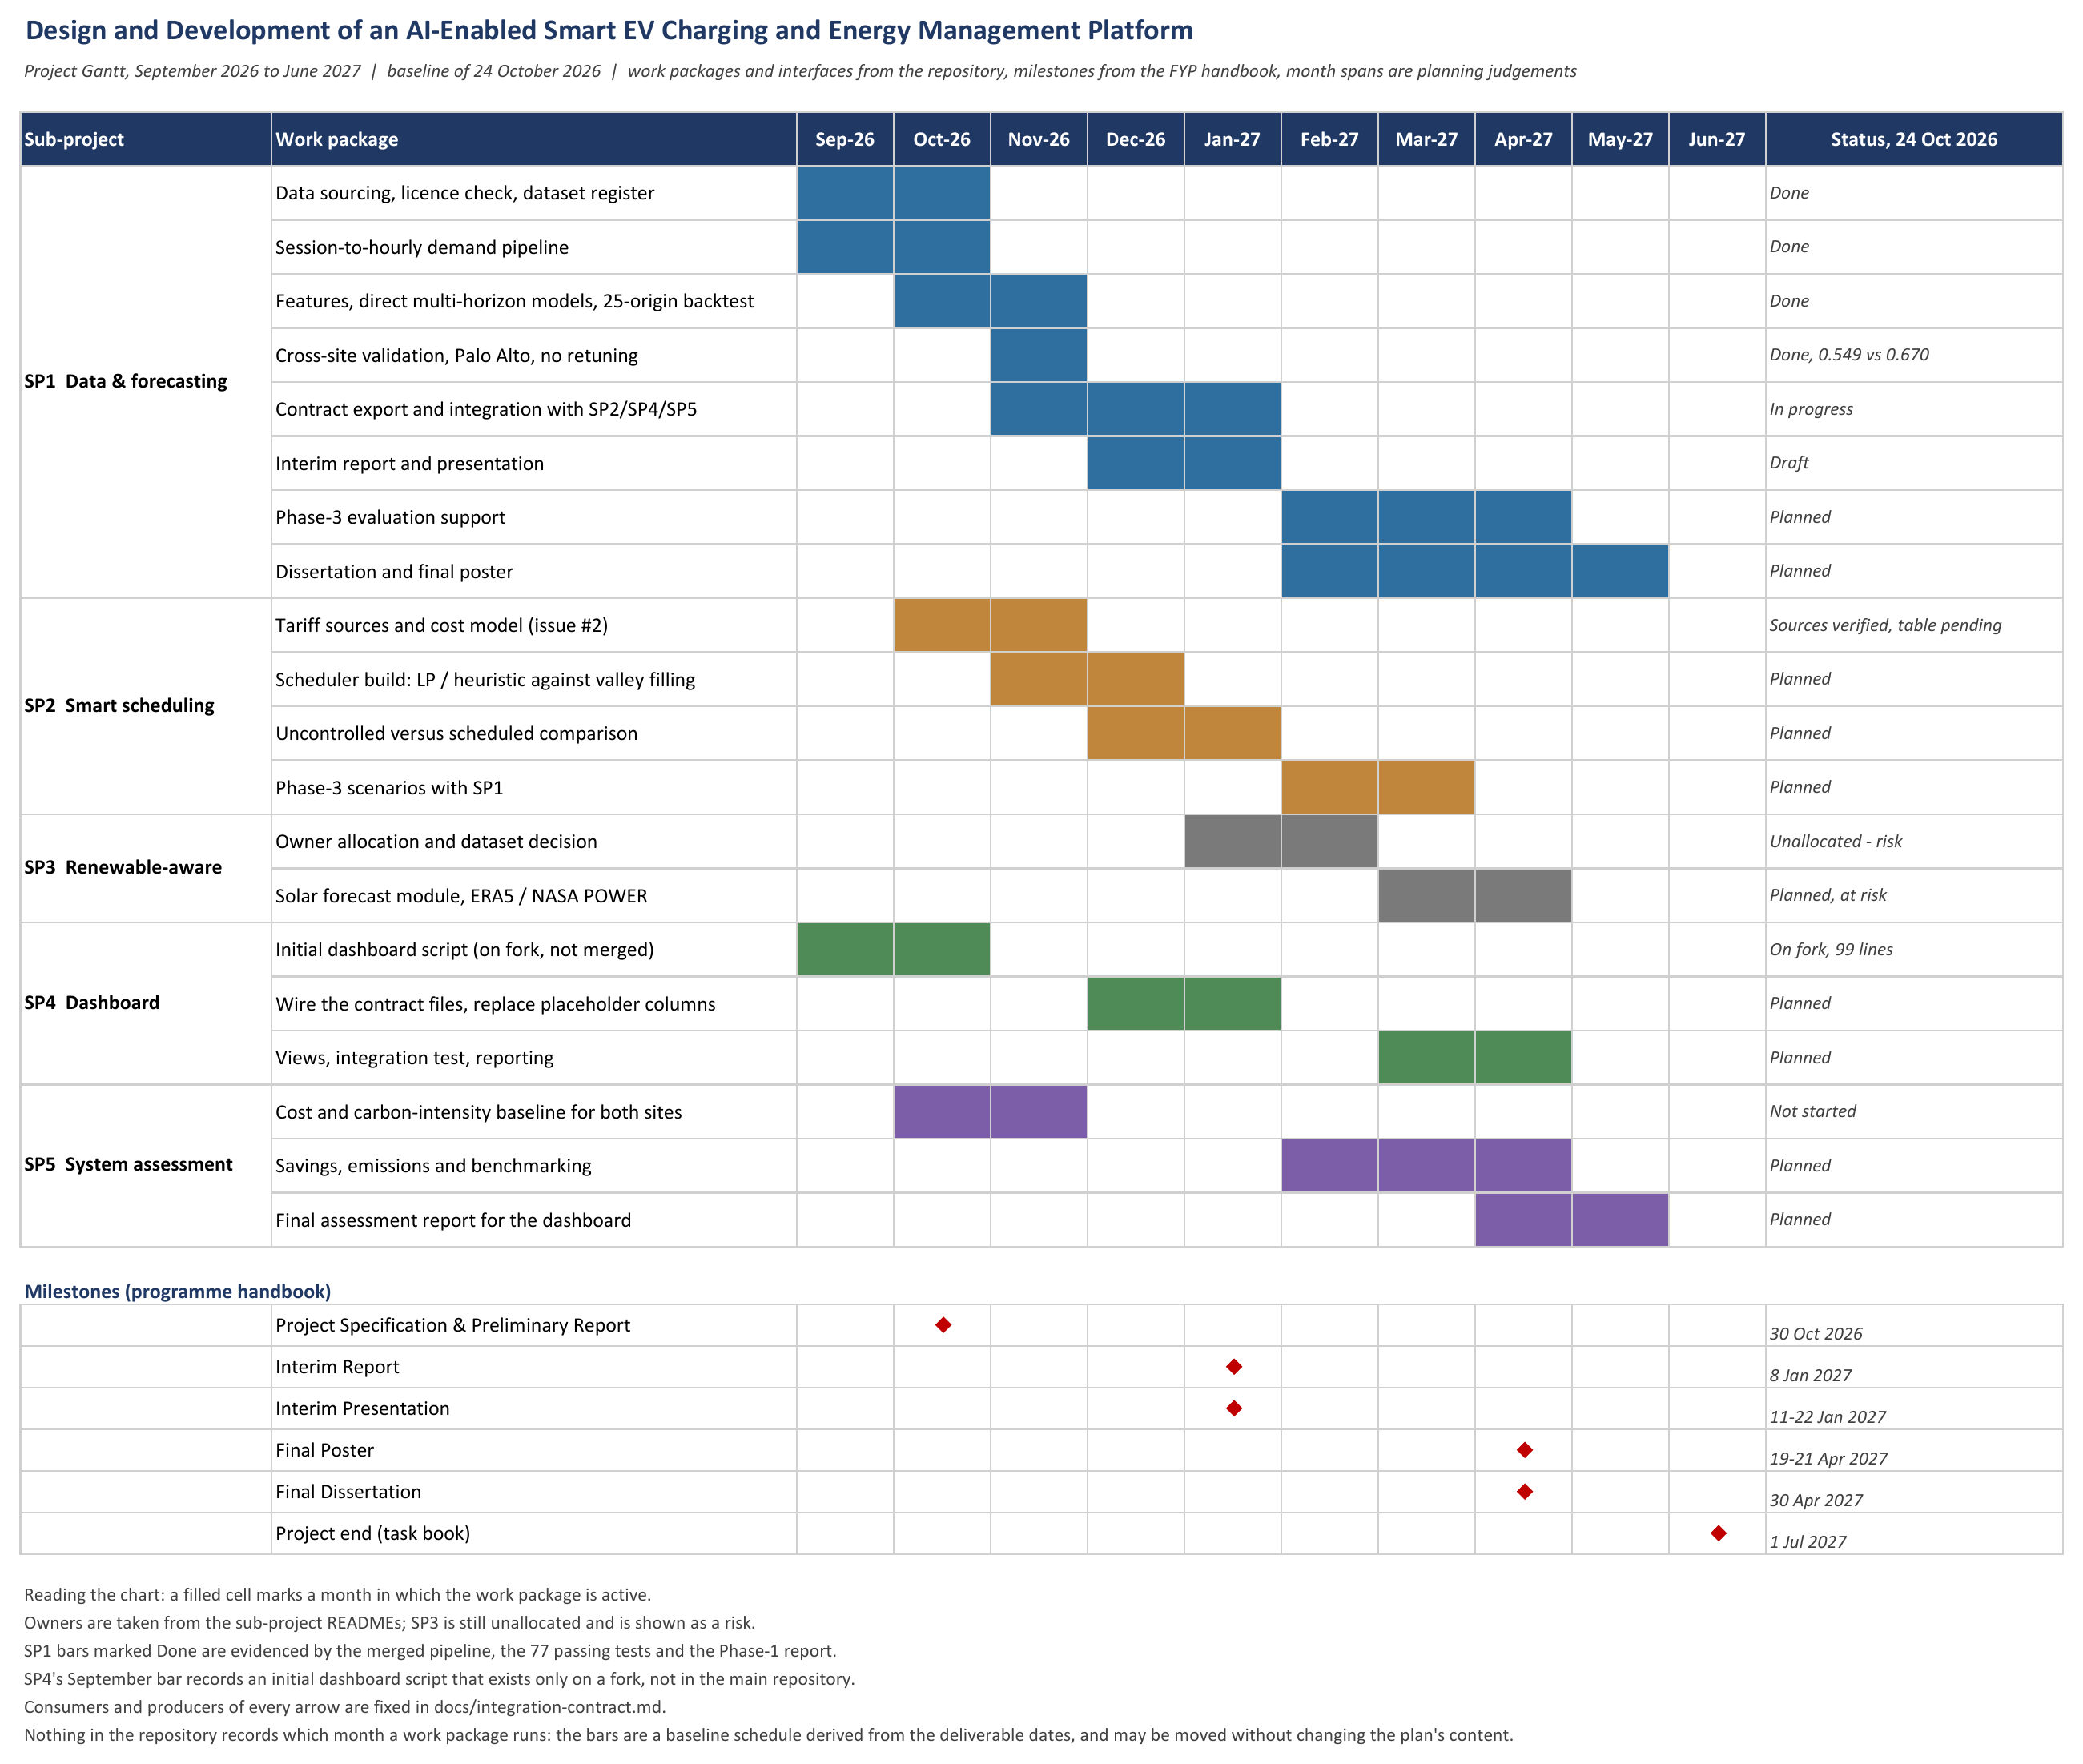
\includegraphics[width=0.86\textwidth]{plan/gantt.png}
\caption{Project Gantt chart, September 2026 to June 2027. Work packages and interfaces come from the
repository, milestone dates from the FYP handbook; the month spans are planning judgements. The
workbook is supplied as \code{gantt.xlsx} so the plan can be edited rather than redrawn.}
\label{fig:gantt}
\end{figure}

\end{document}
